\documentclass[11pt]{article}

\usepackage[a4paper,margin=1in]{geometry}
\usepackage{amsmath,amssymb}
\usepackage{booktabs}
\usepackage{xcolor}
\usepackage{pgfplots}
\pgfplotsset{compat=1.16}
\usepackage[hidelinks]{hyperref}

\title{Heterogeneous Pinned-Expert Placement for DeepSeek V4 Flash\\
\large Streaming avoided and modeled decode/prefill speedup as a function
of pinned expert capacity}
\author{ds4a (fork of antirez/ds4)}
\date{\today}

\newcommand{\gib}{\,\mathrm{GiB}}
\newcommand{\mb}{\,\mathrm{MB}}

\begin{document}
\maketitle

\begin{abstract}
We quantify how much routed-expert streaming is removed by pinning a static
set of experts on a second GPU (e.g.\ an RTX 5060~Ti in a PCIe~3.0$\times$4
slot), and what that implies for decode and prefill speed, as a function of
the pinned capacity. The placement is driven by \emph{measured} per-(layer,
expert) routing frequencies; only the time model is calibrated. All numbers
below come from the scheduler implemented in
\texttt{ds4\_expert\_placement.c} and the CUDA routing profiler.
\end{abstract}

\section{Setup and notation}

The primary GPU (A) is an RTX 3080~Ti on PCIe~4.0$\times$16. It has no room
for a resident expert pool, so every routed expert it executes must be
streamed from host RAM. A second GPU (B) is optional and sits on a slow link
(PCIe~3.0$\times$4); it holds a \emph{static} set of experts in VRAM and never
receives expert weights again after startup. Only small activations cross B's
link.

\begin{center}
\begin{tabular}{ll}
\toprule
Symbol & Meaning \\
\midrule
$s_e$ & bytes per routed expert \\
$K$ & expert selections per generated token ($=43\times 6=258$) \\
$N$ & number of experts pinned on B \\
$C$ & pinned capacity in bytes ($= N s_e$ plus slack) \\
$B_W$ & streaming bandwidth, host RAM $\to$ A \\
$F$ & non-streaming per-token cost on A \\
$\tau$ & per-layer activation exchange cost to B \\
$h_e$ & measured selection count of expert $e$ over a profile \\
$c$ & selection coverage (fraction of decode stream removed) \\
$c_b$ & byte coverage (fraction of prefill stream removed) \\
\bottomrule
\end{tabular}
\end{center}

\section{Expert size}

V4 Flash has 43 layers, 256 routed experts per layer, and selects the top~6
per token. One routed expert is three matmuls whose storage costs follow
directly from the tensor dimensions and the GGUF quantisation bit widths:
\[
\begin{aligned}
\text{gate} &= 4096\cdot 2048 \text{ weights} \times 2.0625\ \text{bit}
            = 17{,}301{,}504\ \text{bit},\\
\text{up}   &= 4096\cdot 2048 \text{ weights} \times 2.0625\ \text{bit}
            = 17{,}301{,}504\ \text{bit},\\
\text{down} &= 4096\cdot 2048 \text{ weights} \times 2.625\ \text{bit}
            = 22{,}020{,}096\ \text{bit}.
\end{aligned}
\]
Summing and converting to bytes,
\[
s_e = \frac{17{,}301{,}504 + 17{,}301{,}504 + 22{,}020{,}096}{8}
    = 7{,}077{,}888\ \text{B} \approx 7.08\mb .
\]
The implementation uses $s_e = 7.07\times 10^{6}$~B.

\section{Bytes and time per token}

Per token the router makes
\[
K = 43 \times 6 = 258
\]
expert selections, so the streamed volume and its transfer time are
\[
V = K\,s_e = 258 \times 7.07\mb = 1.824\ \text{GB},
\qquad
T_{\text{stream}} = \frac{V}{B_W}.
\]

\section{Calibration of the time model}

The baseline is one measurement: the single-GPU decode rate
$r_0 \approx 9.0\ \text{tok/s}$, i.e.
\[
T_0 = \frac{1}{r_0} = 111.1\ \text{ms}.
\]
We split $T_0$ into a streaming part and a fixed part:
\[
T_0 = F + T_{\text{stream}}.
\]
Choosing a stream share of $86\%$ gives
\[
T_{\text{stream}} = 96.0\ \text{ms}
\;\Longrightarrow\;
B_W = \frac{1.824\times 10^{9}\ \text{B}}{96{,}000\ \mu\text{s}}
    \approx 19{,}000\ \text{B}/\mu\text{s}\ (19\ \text{GB/s}),
\]
\[
F = 111.1 - 96.0 = 15.0\ \text{ms}.
\]
The pair $(B_W, F)$ is therefore \emph{the one modeling choice}: it is the
split that reproduces the measured baseline. Everything downstream scales
linearly with it.

\section{Placement: why top-$N$ is optimal}

Given hit counts $h_e$, pin a set $P$ with $|P|=N$ to maximise the removed
selection mass:
\[
\max_{x_e \in \{0,1\}} \sum_e h_e x_e
\qquad \text{s.t.} \qquad \sum_e s_e x_e \le C,\quad \sum_e x_e \le N .
\]
Because every expert has the same size $s_e$, the constraint is a single
cardinality bound: an exchange argument shows the optimum is simply the $N$
experts with the largest $h_e$. The scheduler sorts by $h_e$ and takes the
top $N = \lfloor C/s_e \rfloor$; tiers are filled hottest-GPU-first, then the
second GPU, then RAM, then SSD.

\section{Coverage metrics}

With $P$ the pinned (VRAM) set and $U$ the set of used experts,
\[
c = \frac{\sum_{e\in P} h_e}{\sum_{e\in U} h_e},
\qquad
c_b = \frac{\sum_{e\in P} s_e}{\sum_{e\in U} s_e} = \frac{N}{|U|}.
\]
$c$ is the \emph{selection} coverage: the fraction of the 258 per-token
selections no longer streamed. $c_b$ is the \emph{byte} coverage: in a wide
prefill chunk essentially every used expert is touched, so the prefill stream
is proportional to bytes, not frequency.

\section{Decode model}

Pinned experts are served locally, so the streamed fraction falls to
$(1-c)$. The second GPU additionally requires one activation round trip per
layer \emph{when the token selects one of its experts}. Approximating the six
selections in a layer as independent draws at the layer's mean pinned share
$p_L$,
\[
\Pr[\text{at least one hit in layer } L] = 1-(1-p_L)^{6},
\]
\[
T_{\text{exc}} = \tau \sum_{L=1}^{43}\Bigl(1-(1-p_L)^{6}\Bigr),
\qquad
p_L = \frac{\sum_{e\in P,\,e\in L} h_e}{\sum_{e\in L} h_e}.
\]
The modeled decode time and throughput are then
\[
T_{\text{dec}} = F + T_{\text{stream}}\,(1-c) + T_{\text{exc}},
\qquad
r = \frac{10^{6}}{T_{\text{dec}}\ [\mu\text{s}]}.
\]

\section{Prefill model}

Prefill is compute-bound on A but its expert loading scales with the union of
experts touched, which for a long chunk approaches $U$. Pinning removes a
fraction $c_b$ of that loading, so the modeled prefill speedup of the
expert-stream component is
\[
S_{\text{pre}} = \frac{1}{1-c_b}.
\]
We deliberately do not fold this into a token rate: prefill also has compute,
and B's slow link can bound large chunks.

\section{Results}

Data were collected with the CUDA routing profiler on the RTX 3080~Ti running
V4 Flash IQ2 with SSD streaming. ``Merged'' aggregates three diverse prompts
($\approx 380$ tokens total); ``decode'' is a single generation-heavy run
($\approx 174$ tokens). The second GPU's pinned capacity $C$ is swept from 2
to 64~GiB; the 3080~Ti's own small sticky pool is part of the baseline.

\subsection*{Merged profile (3 prompts)}

\begin{center}
\begin{tabular}{rrrrrr}
\toprule
$C$ [GiB] & $N$ & $c$ [\%] & $c_b$ [\%] & decode t/s & $S_{\text{pre}}$ \\
\midrule
 2 &  303 & 24.71 &  3.88 & 11.29 & 1.04 \\
 4 &  607 & 37.24 &  7.77 & 13.03 & 1.08 \\
 6 &  911 & 46.70 & 11.66 & 14.75 & 1.13 \\
 8 & 1214 & 54.28 & 15.54 & 16.51 & 1.18 \\
12 & 1822 & 66.00 & 23.32 & 20.26 & 1.30 \\
16 & 2429 & 74.63 & 31.09 & 24.35 & 1.45 \\
20 & 3037 & 81.26 & 38.88 & 28.81 & 1.64 \\
24 & 3644 & 86.41 & 46.65 & 33.59 & 1.87 \\
32 & 4859 & 93.51 & 62.20 & 43.58 & 2.65 \\
40 & 6074 & 97.59 & 77.75 & 52.54 & 4.50 \\
48 & 7289 & 99.47 & 93.31 & 58.03 & 14.94 \\
64 & 7812 & 100.00 & 100.00 & 59.81 & -- \\
\bottomrule
\end{tabular}
\end{center}

\subsection*{Decode-heavy profile (single prompt)}

\begin{center}
\begin{tabular}{rrrrrr}
\toprule
$C$ [GiB] & $N$ & $c$ [\%] & $c_b$ [\%] & decode t/s & $S_{\text{pre}}$ \\
\midrule
 2 &  303 & 34.44 &  4.98 & 12.60 & 1.05 \\
 4 &  607 & 47.84 &  9.98 & 15.00 & 1.11 \\
 6 &  911 & 57.22 & 14.98 & 17.33 & 1.18 \\
 8 & 1214 & 64.43 & 19.96 & 19.68 & 1.25 \\
12 & 1822 & 75.14 & 29.96 & 24.64 & 1.43 \\
16 & 2429 & 82.61 & 39.94 & 29.93 & 1.67 \\
20 & 3037 & 88.27 & 49.94 & 35.74 & 2.00 \\
24 & 3644 & 92.40 & 59.92 & 41.64 & 2.50 \\
32 & 4859 & 97.28 & 79.90 & 51.72 & 4.98 \\
40 & 6074 & 99.98 & 99.88 & 59.76 & -- \\
48 & 6081 & 100.00 & 100.00 & 59.81 & -- \\
\bottomrule
\end{tabular}
\end{center}

\begin{figure}[t]
\centering
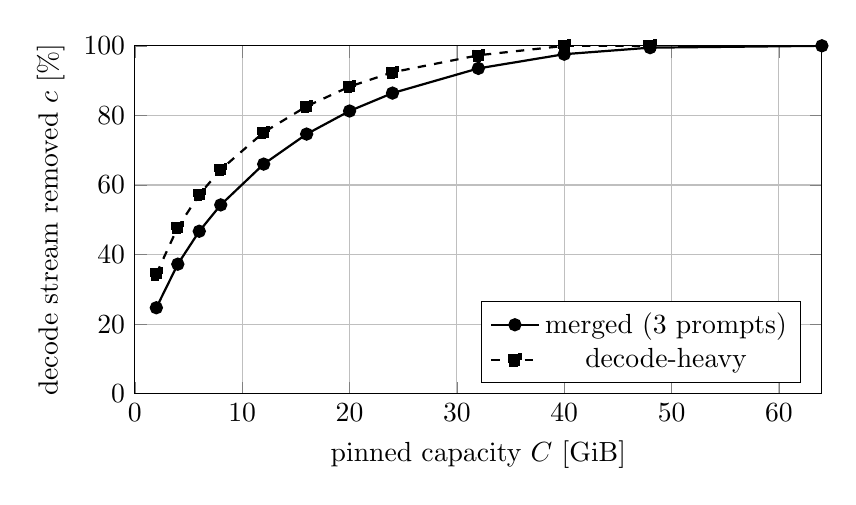
\begin{tikzpicture}
\begin{axis}[
  width=0.85\textwidth, height=6cm,
  xlabel={pinned capacity $C$ [GiB]},
  ylabel={decode stream removed $c$ [\%]},
  xmin=0, xmax=64, ymin=0, ymax=100,
  grid=both, legend pos=south east]
\addplot[thick,mark=*] coordinates {
(2,24.71)(4,37.24)(6,46.70)(8,54.28)(12,66.00)(16,74.63)
(20,81.26)(24,86.41)(32,93.51)(40,97.59)(48,99.47)(64,100.00)};
\addplot[thick,mark=square*,dashed] coordinates {
(2,34.44)(4,47.84)(6,57.22)(8,64.43)(12,75.14)(16,82.61)
(20,88.27)(24,92.40)(32,97.28)(40,99.98)(48,100.00)};
\legend{merged (3 prompts), decode-heavy}
\end{axis}
\end{tikzpicture}
\caption{Selection coverage grows steeply and then saturates: the first
$\sim$16~GiB remove the bulk of the decode stream, later capacity pins
progressively colder experts.}
\end{figure}

\section{Discussion}

\begin{itemize}
\item \textbf{Front-loaded gains.} Coverage is concave. At 16~GiB the merged
profile already removes $c=74.6\%$ of the decode stream (modeled $9.0\to
24.4$~t/s); doubling to 32~GiB adds only $\sim$19 points.
\item \textbf{Decode vs prefill.} Decode benefits from routing skew ($c$ up
to $99\%$), whereas prefill is proportional to pinned bytes ($c_b$), so the
same placement removes far less prefill stream ($31\%$ at 16~GiB).
\item \textbf{Saturation.} As $c\to 1$ the stream term vanishes and
$T_{\text{dec}}\to F+T_{\text{exc}}$, i.e.\ $\approx 60$~t/s. The model
should not be trusted at that extreme: once A is no longer the bottleneck,
B's own compute and its $\times4$ link become the limit, which this model
does not represent.
\item \textbf{Workload dependence.} Single-prompt profiles show higher
coverage than the merged one ($82.6\%$ vs $74.6\%$ at 16~GiB). A broad corpus
would be lower still. The tool consumes real profiler counts, so this is
measurable rather than assumed.
\item \textbf{Why B's slow link is acceptable.} A resident expert is read
from B's VRAM in $\sim$$16\ \mu$s, versus $\sim$$470\ \mu$s to stream it to A;
B is therefore never the decode critical path, and its link carries only
small activations.
\end{itemize}

\section{Reproducing}

\begin{verbatim}
make test-expert-placement
# collect real routing counts on CUDA:
DS4_EXPERT_HOTLIST=/tmp/p.hotlist ./ds4 -m ds4flash.gguf --cuda \
    --ssd-streaming --ssd-streaming-cache-experts 1GB --ctx 512 \
    --nothink -p "..." --tokens 150
# capacity sweep:
./tests/test_expert_placement --sweep /tmp/p.hotlist
\end{verbatim}

\end{document}
